% \chapter{Multi-task learning with Machine Translation}

% \section{POS Tagging}
% By introducing linguistic information to the model, we hypothesize that the original model was not able to extract this information from raw text, and explicitly feed the model with such information will improve it. However, in the unfortunate event that the translation model has already captured the information of POS tags, it might be helpful to use these attention layers to do POS tagging.

\chapter{Promoting Dependency Interpretation of Self-Attention to Jointly Parse and Translate}

\section{Graph-base Dependency Parser}

\section{Parsing from Transformer's Self-Attention Weights}

\cite{DBLP:journals/corr/DozatM16} proposed a graph-based dependency parsing model, in which the output matrix S contains information S(u, v): the probability that u is the head of v.
This matrix is similar to the idea of the attention scores $\alpha$ in attention model, hence, we could attempt to combine this model and the translation model:
\begin{itemize}
    \item Train the mixed model simultaneously to perform 2 tasks.
    \item Use the matrix S from parsing sub-model as the self-attention weight in the encoder of the MT sub-model.
\end{itemize}


In this section, we propose a different but similarly simple technique to
promote the explicit knowledge of source syntax in the model. Our inspiration
comes from
the neural model for dependency parsing by
\perscite{DBLP:journals/corr/DozatM16}. The model produces a matrix $S(u, v)$
expressing the probability that the word $u$ is the head of $v$. The
construction of this matrix is very similar to the matrix of self-attention weights $\alpha$ in the Transformer
model. From this similarity, we speculate that the self-attentive architecture
of Transformer NMT
has the capacity to learn dependency parsing and we only need to promote a
little the particular linguistic dependencies captured in a treebank.

Our joint model is inspired by the similarity of a graph-based neural network dependency parser \cite{DBLP:journals/corr/DozatM16} and the self-attention weights in the encoder of the Transformer \cite{DBLP:conf/nips/VaswaniSPUJGKP17}.

\begin{figure}
    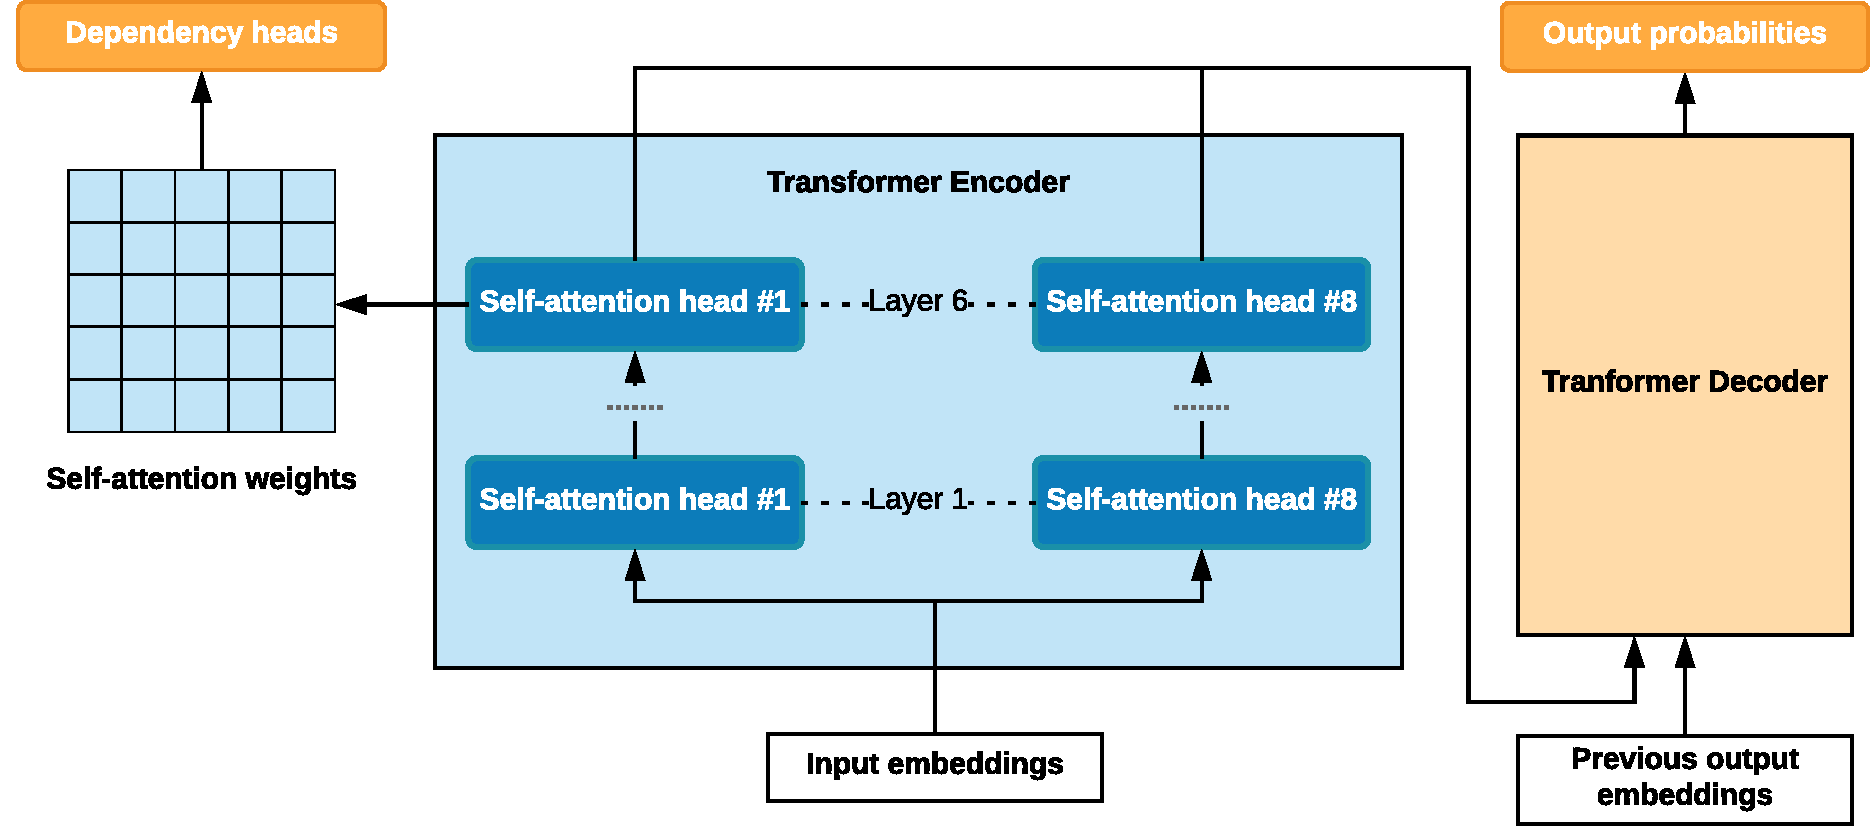
\includegraphics[width=\linewidth]{img/Joint_Translation_DepParse}
    \caption{Joint dependency parsing and translation model}
    \label{fig:joint_trans_depparse}
\end{figure}

\cref{fig:joint_trans_depparse} illustrates our joint model. The translation
part is kept as is. The only difference is that we reuse one of the
self-attention heads in the Transformer encoder and reinterpret it as if it was
the dependency matrix $S(u, v)$. The training objective is combined and
maximizes both the translation quality in terms of cross-entropy of the
candidate translation and the unlabeled attachment score (UAS) of the proposed
heads against the golden parse.\footnote{It should be noted that the dependency
parses we use are actually automatic, produced by
\perscite{mcdonald:pereira:ribarov:hajic:2005} parser incorporated in the Treex
platform formerly known as TectoMT \parcite{tectomt:popel:2010};
\url{http://ufal.mff.cuni.cz/treex}.}

The particular choice of the head which will serve as the dependency parser is
arbitrary. Put differently, we constrain the Transformer model to use one of its
heads to follow the given syntactic structure of the sentence. It would be also
possible to use e.g. the deep-syntactic parse of the sentence (the
tectogrammatical layer as defined e.g. for the Prague Dependency Treebank,
\inparcite{pdt20:2006}); we leave that for future work.
